\documentclass{beamer}
\usepackage{amsmath}
\usepackage{graphicx}
\usepackage{amssymb}
\usepackage{hyperref}
\newcommand{\nand}{\uparrow}

\title{MATH1061 Week 3 Tutorial}
\date{12 March 2013}

\begin{document}

\frame{\titlepage}

\begin{frame}
\frametitle{Valid arguments}
\end{frame}

\begin{frame}
% Note to self: scrap this question.
\frametitle{Digital Logic}

If $p$ and $q$ are statement forms, we define the {\bf alternative denial} of
$p$ and $q$ to be $\sim (p \land q)$, written $p \nand q$, said ``$p$ nand $q$''.
In building digital circuits, it is easy to build a NAND-gate out of transistors,
and then we can build other gates (AND, OR, NOT) out of multiple NAND-gates.

\centering
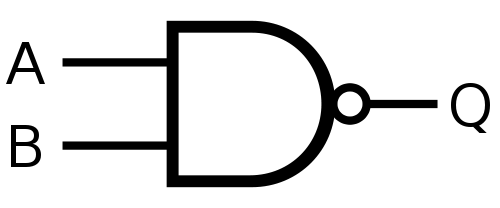
\includegraphics[width=0.3\textwidth]{src/nand.png}

\begin{enumerate}
\item Write a statement form equivalent to $\sim p$, using only $\nand$.
\item Write a statement form equivalent to $p \land q$, using only $\nand$.
\item Write a statement form equivalent to $p \lor q$, using only $\nand$.
\item (Bonus) Draw your answers to the above as digital logic circuits.
\end{enumerate}

\end{frame}

\end{document}
